\documentclass{exam}

\usepackage{amsmath,amssymb,amsfonts,amsthm,dsfont}
\usepackage{lib/extra}
\usepackage{graphicx}
\usepackage{tikz}
\usepackage{enumitem}
\usepackage{bbm}
\usepackage{pgfplots}
\usepackage{fontenc}
\usepackage{float}

\pgfplotsset{compat=1.18}
\renewcommand{\arraystretch}{1.5}
\setcounter{section}{2}

\title{Complex Analysis Chapter 1 Section 3}
\author{Brandyn Tucknott}
\date{Last Updated: 29 September 2025}

\begin{document}
\maketitle

\section{Integration along curves}
A \textbf{parameterized curve} $z(t)$ which maps a closed interval $[a, b] \subset \R$ to the complex plane. We say that the parameterized
curve is \textbf{smooth} if $z'(t)$ exists and is continuous on $[a, b]$ with $z'(t) \neq 0$ for $t\in [a ,b]$. At the points $t = a, b$,
$z'(a), z'(b)$ are interpreted as one-sided limits:
$$z'(a) = \lim_{h\to 0, h > 0} \frac{z(a + h) - z(a)}{h} \text{ and } z'(b) = \lim_{h\to 0, h < 0} \frac{z(b + h) - z(b)}{h}.$$
These quantities are called the right-handed derivative at $z(a)$ and left handed derivative at $z(b)$. We say the parameterized curve is
\textbf{piecewise-smooth} if $z$ is continuous on $[a, b]$ and there exist points $a = a_0 < a_1 < \hdots < a_n = b$,
where $z(t)$ is smooth on the intervals $[a_k, a_{k + 1}]$. The right-handed derivative and left-handed derivative at $a_k$ may differ for 
$k = 1, 2, \hdots, n - 1$.

Two parameterizations
$$z: [a, b]\to\C \text{ and } \tilde{z}: [c, d]\to \C$$
are \textbf{equivalent} if there exists a continuously differentiable bijection $s\to t(s)$ from $[c, d]\to[a, b]$ so that $t'(s) > 0$ and
$$\tilde{z}(s) = z(t(s)).$$

The condition $t'(s) > 0$ says that orientation must be preserved: as $s$ travels from $c$ to $d$, $t(s)$ travels from $a$ to $b$. The points
$z(a)$ and $z(b)$ are called \textbf{end-points} of the curve and are independent on the parameterization. Since a curve $\gamma$ carries an
orientation, it is natural to say that $\gamma$ begins at $z(a)$ and ends at $z(b)$. A smooth or piecewise-smooth curve is \textbf{closed}
if $z(a) = z(b)$ for any of its parameterizations, and \textbf{simple} if it is not self-intersecting ($z(t) \neq z(s)$ unless $s = t$).

\begin{figure}[H]
    \centering
    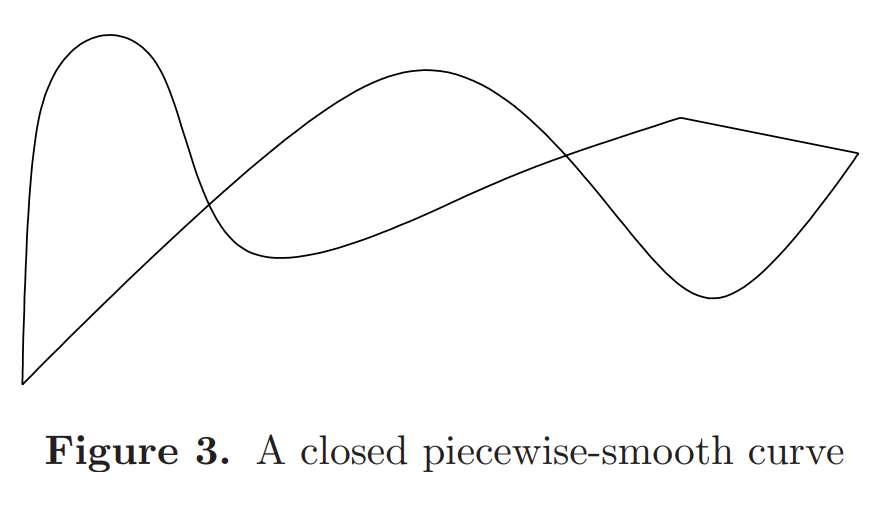
\includegraphics[width=0.5\textwidth]{figures/complex_analysis/figure_3.png}
\end{figure}

We will call any piecewise-smooth curves a \textbf{curve}, since these are our objects of primary concern. A basic example is a circle
centered at $z_0$ with radius $r$, which is by definition
$$C_r(z_0) = \cbrac{z\in\C : |z - z_0| < r}.$$

The \textbf{positive orientation} (counterclockwise) is one given by the standard parameterization
$$z(t) = z_0 + re^{it}\text{ where } t\in[0, 2\pi],$$
while the \textbf{negative orientation} (clockwise) is the one given by 
$$z(t) = z_0 + re^{-it}\text{ where } t\in[0, 2\pi].$$

In the following chapters, we denote by $C$ the general positively oriented circle. Loosely speaking, a key theorem in complex analysis
states that if a function is holomorphic is the interior of a closed curve $\gamma$, then
$$\int_\gamma f(z) dz = 0. \text{ (we explore this more next chapter)}$$

Given a smooth curve $\gamma$ in $\C$ parameterized by $z: [a, b]\to \C$, and $f$ a continuous function on $\gamma$, we define the integral
of $f$ along $\gamma$ as
$$\int_\gamma f(z)dz = \int_a^b f(z(t))z'(t)dt.$$

For this definition to have meaning, we have to show that the right-hand integral is independent the choice of $\gamma$. Say that $\tilde{z}$
is an equivalent parameterization as above. Then the change of variables formula and chain rule imply that
$$\int_a^b f(z(t))z'(t)dt = \int_c^d f(z(t(s)))z'(t(s))t'(s)ds = \int_c^d f(\tilde{z(s)})\tilde{z}'(s)ds.$$
Thus the integral of $f$ over $\gamma$ is well-defined.

If $\gamma$ is piecewise-smooth and $z(t)$ a piecewise-smooth parameterization, then
$$\int_\gamma f(z) dz = \sum_{k = 0}^{n - 1}\int_{a_k}^{a_{k + 1}} f(z(t))z'(t)dt. $$
By definition, the length of a smooth curve $\gamma$ is 
$$\text{length}(\gamma) = \int_a^b \abs{z'(t)}dt. $$
If $\gamma$ is piecewise smooth, the its length is the sum of its smooth parts.

\noqed
\begin{proposition}
    Integration of continuous functions over curves satisfies the following properties:
    \begin{itemize}
        \item It is linear, that is, if $\alpha, \beta\in\C$, then
        $$\int_\gamma \alpha f + \beta g = \alpha \int_gamma f + \beta \int_\gamma g$$

        \item If $\gamma^-$ is $\gamma$ with the reverse orientation, then
        $$\int_\gamma f = -\int_{\gamma^-} f$$

        \item One has the inequality
        $$\abs{\int_\gamma f} \leq \sup_{z\in\gamma} \abs{f(z)}\cdot\text{length}(\gamma)$$
    \end{itemize}
\end{proposition}
\yesqed

\begin{proof}
    The first property follows from linearity of the Riemann integral. The second property (left as exercise: TODO). For the third property,
    note that
    $$\abs{\int_\gamma} f \leq \sup_{t\in[a, b]}\abs{f(z(t))}\int_a^b |z'(t)|dt \leq \sup_{z\in\gamma} \abs{f(z)} \cdot \text{length}()\gamma$$
    as was to be shown.
\end{proof}

A \textbf{primitive} for $f$ on $\Omega$ is a function $F$ that is holomorphic on $\Omega$ and such that $F'(z) = f(z)$ for all $z\in\Oemga$. 
\noqed
\begin{theorem}\label{thm:main}
    If a continuous function $f$ has a primitive in $\Omega$, and $\gamma$ is a curve in $Omega$ that begins at $w_1$ and ends at $w_2$, then
    $$\int_\gamma f(z) dz = F(w_2) - F(w_1).$$
\end{theorem}
\yesqed
\begin{proof}
    If $\gamma$ is smooth, then by application of the chain rule and the fundamental theorem of calculus it is true. If $z: [a, b]\to\C$
    is a parameterization of $\gamma$, then $z(a) = w_1$ and $z(b) = w_2$ and we have
    \begin{align*}
        \int_\gamma f(z)dz &= \int_a^b f(z(t))z'(t)dt \\
        &= \int_a^b F'(z(t))z'(t)dt \\
        &= \int_a^b \frac{d}{dt} F(z(t))z'(t)dt \\
        &= F(z(b)) - F(z(a)).
    \end{align*}

    If $\gamma$ is only piecewise-smooth, then we can obtain the telescopic sum
    \begin{align*}
        \int_\gamma f(z)dz &= \sum_{k = 0}^{n - 1}F(z(a_{k + 1})) - F(z(a_k)) \\
        &= F(z(a_n)) - F(z(a_0)) \\
        &= F(z(b)) - F(z(a))
    \end{align*}
\end{proof}

\noqed
\begin{corollary}
    If $\gamma$ is a closed curve in an open set $\Omega$, and $f$ is continuous and has a primitive in $\Omega$, then 
    $$\int_\gamma f(z) dz = 0.$$
\end{corollary}
\begin{corollary}
    If $f$ is holomorphic in a region $\Omega$ and $f' = 0$, then $f$ is constant.
\end{corollary}
\yesqed
\begin{proof}
    Fix a point $w_0\in\Omega$. It suffices to show that $f(w) = f(w_0)$ for all $w\in\Omega$. Since $\Omega$ is connected, for any $w\in\Omega$,
    there exists a curve $\gamma$ which joins $w_0$ to $w$. Since $f$ is clearly a primitive for $f'$, we have
    $$\int_\gamma f'(z)dz = f(w) - f(w_0).$$
    By assumption, $f' = 0$ so the integral on the left is 0, and we conclude that $f(w) = f(w_0)$.
\end{proof}

\textbf{Remark on notation. } When convenient, we follow the practice of using the notation $f(z) = O(g(z))$ to mean that there is a 
constant $C > 0$ such that $|f(z)| \leq C|g(z)|$ for $z$ in the neighborhood of the point in question. In addition, we say $f(z) = o(g(z))$
when $|f(z) / g(z)|\to 0$. We also write $f(z)\sim g(z)$ to mean that $f(z) / g(z)\to 1$. 

\end{document}